\documentclass[twoside]{article}
\usepackage{amsgen,amsmath,amstext,amsbsy,amsopn,amssymb,}
\usepackage{graphicx}
\usepackage{epsfig}

\setlength{\oddsidemargin}{0.1 in} \setlength{\evensidemargin}{-0.1
in} \setlength{\topmargin}{-0.6 in} \setlength{\textwidth}{6.5 in}
\setlength{\textheight}{10.5 in} \setlength{\headsep}{0.1 in}
\setlength{\parindent}{0 in} \setlength{\parskip}{0.1 in}

\newcommand{\homework}[2]{
   \pagestyle{myheadings}
   \thispagestyle{plain}
   \newpage
   \setcounter{page}{1}
   \noindent
   \begin{center}
   \framebox{
      \vbox{\vspace{2mm}
       \hbox to 6.28in { {\bf Math 4720:~Statistical Methods \hfill} }
       \vspace{6mm}
       \hbox to 6.28in { {\Large \hfill #1 (#2)  \hfill} }
       \vspace{6mm}
      \vspace{2mm}}
   }
   \end{center}
   \markboth{#1}{#1}
   \vspace*{4mm}
}

\newcommand{\bbF}{\mathbb{F}}
\newcommand{\bbX}{\mathbb{X}}
\newcommand{\bI}{\mathbf{I}}
\newcommand{\bX}{\mathbf{X}}
\newcommand{\bY}{\mathbf{Y}}
\newcommand{\bepsilon}{\boldsymbol{\epsilon}}
\newcommand{\balpha}{\boldsymbol{\alpha}}
\newcommand{\bbeta}{\boldsymbol{\beta}}
\newcommand{\0}{\mathbf{0}}

\begin{document}

\homework{$4^{th}$ Week Summary}{02/06/25}
\vspace{-0.2 in}
\begin{itemize}
\item A \textbf{Normal} distribution is described by a Normal density curve. We will say $X\sim N(\mu,\sigma^2)$, and the normal density function is given by: $f(x)=\dfrac{1}{\sqrt{2\pi\sigma^2}}\exp\Biggl(-\dfrac{(x-\mu)^2}{2\sigma^2}\Biggr)$
\item The $68\textrm{-}95\textrm{-}99.7$ Rule (a.k.a \textbf{the Empirical Rule})
\item The standardized value is called a z-score. $z=\dfrac{x-\mu}{\sigma}$
\item Finding Normal Probabilities :
\subitem Less than: $P(X<x)=P\Bigl(\dfrac{X-\mu}{\sigma}<\dfrac{x-\mu}{\sigma}\Bigr)=P(Z<z)$
\subitem Greater than: $P(X>x)=P(Z>z)=1-P(Z<z)$
\subitem Between two numbers: $P(a<X<b)=P(z_a<Z<z_b)=P(Z<z_b)-P(Z<z_a)$
\subitem Outside two numbers:
\subitem $P(X < a \bigcup X > b)=P(Z < z_a \bigcup Z > z_b)=1-P(z_a<Z<z_b)=P(Z<z_a)+1-P(Z<z_b)$
\item The \textbf{sampling distribution} of a statistic is the distribution of values taken by the statistic in all possible samples of the same size from the same population
\item If \textit{individual observations} have the $N(\mu,\sigma^2)$ distribution, then the \textit{sample mean} of a random sample of size $n$ has the $N(\mu,\dfrac{\sigma^2}{n})$ distribution.
\item \textbf{CLT} (Central Limit Theorem): Draw a random sample of size $n$ from any population with mean $\mu$ and finite standard deviation $\sigma$. When $n$ is large, the sampling distribution of the sample mean is approximately $N(\mu,\dfrac{\sigma^2}{n})$.
\item Means of \textit{random samples} are \textbf{less variable} than \textit{individual observations}.
\item Means of \textit{random samples} are \textbf{more normal} than \textit{individual observations}.
\item The probability that the sample mean $\bar{x}$ is close to $\mu$ increases as the sample size $n$ becomes large. This is commonly referred to as the \textbf{Law of Large Numbers}.
\begin{figure}[h]
\begin{center}
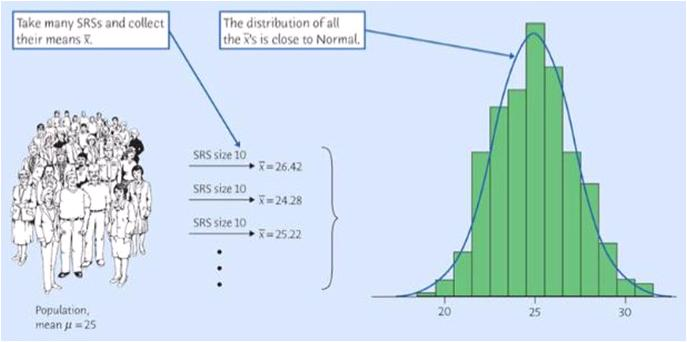
\includegraphics[angle=0, width=14 cm] {sample_mean.jpg}
\end{center}
\end{figure}
\end{itemize}
\end{document}


